\documentclass[conference]{IEEEtran}
\IEEEoverridecommandlockouts
\usepackage{graphicx}
\usepackage{algorithm}
\usepackage{algorithmicx}
\usepackage{algpseudocode}
\usepackage[dvipsnames]{xcolor}
\usepackage{amsmath}
\usepackage{hyperref}

\algblock{Input}{EndInput}
\algnotext{EndInput}
\algblock{Output}{EndOutput}
\algnotext{EndOutput}
\newcommand{\Desc}[2]{\State \makebox[2em][l]{#1}#2}

\newcommand{\tristan}[1]{\color{orange}\textbf{From Tristan:}#1\color{black}}


\begin{document}
\title{I/O simulation model with Linux page cache, integration and evaluation in SimGrid framework}

\author{\IEEEauthorblockN{Hoang-Dung Do, Tristan Glatard and Val\'erie Hayot-Sasson
  }\\
  \IEEEauthorblockA{
    Department of Computer Science and Software Engineering, Concordia University, Montreal, Canada
  }
}

\maketitle

	\begin{abstract}
		\begin{itemize}
			\item The I/O bottleneck in HPC and the need of experiments.
			\item HPC experiment frameworks and advantages of SimGrid.
			\item The missing of the ability to simulate page cache, the goal of this paper.
			\item Principle of the simulator, experiment scenarios and comparisons.
			\item Brief discussion on results and future work.
		\end{itemize}
	\end{abstract}

	\section{Introduction}
		\begin{itemize}
			\item HPC, the bottleneck in I/O and the demand of HPC experiments. 
			\item Difficulties in conducting high performance computing experiments and the need of simulation frameworks.
			\item Existing experiment methods, simulators, simulation frameworks. The advantages of SimGrid compared to others \cite{casanova2008, lebre2015}. The missing of the ability to simulate page cache in SimGrid \cite{lebre2015}.
			\item The objective of the paper: Add capability to simulate I/O with page cache in SimGrid.
		\end{itemize}
	\section{Related Work}			
		
		\subsection{Page cache}
			\begin{itemize}
				\item What is page cache? How it works \cite{linuxdev3rd2010}. Effects and importance of page cache.
				\item Introduce some existing strategies with some highlighted pros and cons.
				\item Current implementation in Linux and some reasons why it is chosen to be implemented (implementation complexity, effectiveness, overhead, etc) \cite{linuxdev3rd2010}
			\end{itemize}									

		\subsection{Simulators}
			\begin{itemize}
				\item Discuss some existing methods, simulation frameworks to conduct HPC experiments. Compare pros and cons (accuracy, simulation time, usability) of some simulators (SimGrid, GridSim).
				\item Related development: RAM energy consumption \cite{gill2019} \cite{ouarnoughi2017} 
				\item Discuss the pros of SimGrid and the reasons why we chose it to extend. (Section 2.2.2 in \cite{casanova2014})
			\end{itemize}
			
	\section{Method}
		In this section, we discuss our approach to model page cache and
		the cache eviction strategy implemented in Linux. We also detail
		the design the simulators in order to generalize page cache as well
		as the implementation in Python and SimGrid framework. Finally, we
		describe some experimental scenarios to compare the results of
		Python simulator, baseline SimGrid simulator and the results from
		the real pipelines. 

		\subsection{Principle of the simulator}
	
			When modeling the I/O time, we consider the key factors of the
			I/O mechanism having the biggest impacts on data read/write.
			The first factor taken into account is the use of the page
			cache in Linux kernel. The second factor  is the cache eviction, 
			data flushing and cache eviction mechanisms implemented in the 
			Linux kernel, as they manage and change the status of the memory 
			including cache size, amount of available memory and 
			dirty data, based on which the kernel controls I/O activities. Therefore, 
			the idea of our simulator is to simulate the memory, the Linux 
			page cache with its LRU lists, storage device and imitate the data flushing 
			and cache eviction algorithm implemented in the kernel. 
			
			At the level of detail in our simulator, the simulation models of memory 
			and storage devices are straightforward when they can be modeled with 
			predefined capacity and bandwidth. To simulate the cache eviction mechanism 
			implemented in Linux, our simulator also keeps tracks of page cache 
			LRU lists as in the kernel. However, instead of dealing with lists pages, we 
			consider a sequence of continuously accessed pages of a file as a single 
			unit, a block of data. A data block keeps the information about file name, 
			block size, last access and a dirty flag describing whether the data is 
			dirty or not. 
			
			The idea of data block offers our simulator some obvious advantages. 
			In cache eviction algorithm, which is one of the key components 
			in our model, maintaining and handling pages in packet level are 
			non-trivial when they require significant implementation overhead and 
			would likely to hinder the performance of the simulator. The concept of data 
			block not only simplifies our cache eviction simulation but also allows to 
			preserve the accuracy of the simulator by using a single page as the 
			representative for a sequence of pages with similar properties including 
			file name, last access, dirty or not. Because a block represents a set of 
			pages in real systems, it can be split if some data needs to be moved 
			between the page cache LRU lists or evicted from cache. However, blocks can 
			not be merged as we want to preserve this level of granularity to maintain 
			high accuracy.			 
			
			Having these simulation components, we can generalize I/O activities in
			our simulator. When the kernel reads and writes data, it simply 
			reads/writes data from/to disk or cache with predefined disk bandwidth 
			or memory bandwidth. The data blocks are added or updated in page cache 
			LRU lists accordingly. In flushing and periodical flushing, the kernel 
			traverses through the inactive and active lists to reduce the amount of 
			dirty data, while cache eviction algorithm deletes blocks from the 
			inactive list. The page cache LRU lists are updated after every I/O action.
			
			\begin{figure}
   				\centering
   				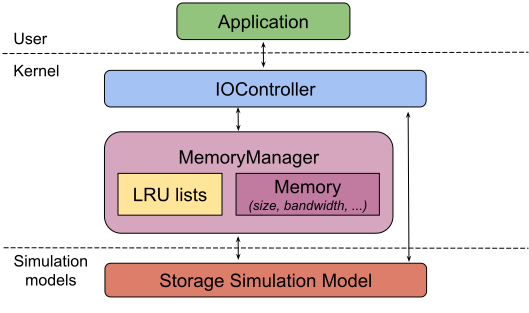
\includegraphics[width=0.85\columnwidth]{figures/interaction.pdf}
   				\caption{The additional layer between user application layer and 
   				original SimGrid API}\label{fig:interaction}
			\end{figure}			
			
			We encapsulate our simulation components with kernel-like functionalities 
			into a layer between user simulated application and storage simulation 
			component (Figure~\ref{fig:interaction}). Our new layer includes two main
			classes, the \textbf{\textit{IOController}}, which models the kernel 
			I/O controlling logic, and the \textbf{\textit{MemoryManager}}, which 
			manages page cache LRU lists and stores all necessary information about 
			memory including capacity, amount of cache, amount of memory used 
			by applications. Because every node has its own memory, storage devices 
			and system configurations, there is one IOController object and one 
			MemoryManager object created for each node. The IOController class 
			keeps system parameters (dirty{\_}ratio, dirty{\_}background{\_}ratio), 
			implements necessary I/O control functionalities such as read, write,
			flushing, and cache evicting. 

			With this layer, user simulated applications send requests to an 
			IOController of the node where requested data is stored, instead of 
			sending read/write requests directly to storage model as in simulators 
			with the current SimGrid version. Based on the memory status in 
			MemoryManager, the IOController orchestrates cache read/write, 
			disk read/write, flushing and cache eviction to fulfill application 
			requests. The time for each action is estimated and the total time of 
			a request is returned to user applications.
			
			\begin{algorithm}\caption{Read}\label{alg:read}
				\small
				\begin{algorithmic}[1]
					\Input
        				\Desc{fn}{file name}
        				\Desc{fs}{file size}
						\Desc{rt}{current simulated run time}
						\Desc{mm}{MemoryManager object}
						\Desc{$r_m$}{memory read bandwidth}
						\Desc{$r_d$}{disk read bandwidth}
   					\EndInput
   					\Output
						\Desc{rt}{simulated run time after the file is read}
   					\EndOutput
					\State mem\_required = max(0, 2 * fs - mm.cached\_data(fn) - 
					mm.available\_memory()) 
					\State mem\_avail = max(0, 2 * fs - mm.cached\_data(fn) - 
					mm.dirty\_data())
					\State rt = rt +  mm.flush(mem\_required - 
					mem\_avail)	
					\State free\_mem\_required = max(0, 2 * fs - mm.cached\_data(fn) - 
					mm.free\_memory())
					\State mm.evict(free\_mem\_required) 
					\If {mm.cached\_data(fn) $>$ 0}
    					\State mm.cache\_read(fn) 
						\If {mm.cached\_data(fn) == fs}
    						\State time = mm.cache\_data(fn) / $r_m$
    						\State IOController.periodic\_flush(time) 
							\State rt = rt + time
						\EndIf
					\EndIf
					\If {mm.cached\_data(fn) $<$ fs}
						\State rt = rt + IOController.flush(mm.dirty\_data())
						\State mm.disk\_read(fs - mm.cache\_data(fn), fn)
    					\State rt = rt + (fs - mm.cache\_data(fn)) / $r_d$
					\EndIf					
					
					\Return rt
					
				\end{algorithmic}
			\end{algorithm}			
			
			The algorithm to generalize file read is described in 
			\textit{Algorithm~\ref{alg:read}}. In Linux systems, data can be read in 
			two ways, read from cache with memory bandwidth and read from disk 
			with disk bandwidth. Because total read time can be seen as a 
			linear function of the read time in each of these two modes, 
			we can generalize reading process as two separate and sequential phases, 
			one is cache read, and the other is disk read. When a user application 
			requests a file read, it calls the read method of the IOController. Then, 
			IOController calculates how much memory is required to read the file 
			based on the amount of available memory, file size, and the amount of 
			file data cached (line 10). If there is not enough available memory, 
			dirty data is flushed to disk to make more memory available by calling flush
			function with the amount of memory needed as the parameter (line 11-12).
			IOController then evicts old blocks from the inactive list to
			accommodate the requested file and flushing time is simulated (line 13-14). 
			After that, IOController starts estimating file read time by first checking 
			if a some file data is cached (line 15). If there is cached data, 
			it is read from cache and the blocks containing this data are updated in 
			the page cache LRU lists with the last access time (line 16). If all file data 
			is cached, time to read from cache is added to total run time, and 
			periodical flushing is triggered to flush dirty data during the cache read 
			(line 18-19). If only a part of the file is in cache, disk read is required, 
			this does not allow flushing and makes the cache read time neglectable. 
			At the beginning of a disk read, dirty data is flushed, then data is read 
			and added to the inactive list, disk read time is estimated with disk read 
			bandwidth and added to total run time (line 23-27). 

			\textit{Algorithm~\ref{alg:write}} describes our
			generalization of file write. Similar to the file read process,
			a file can also be written with two different bandwidths,
			memory bandwidth and disk bandwidth, and thus file write can be
			generalized with two modes. File can be written with memory
			bandwidth before the page cache is saturated, or the amount of
			dirty data reaches dirty\_ratio. Firstly, if dirty\_ratio is not reached 
			the amount of data can be written with memory bandwidth is
			calculated with the formula:
			\begin{equation}
				M = max(0, \frac{(d*C - D)*w_m}{w_m - w_d})\label{equa:freeamt}
			\end{equation}			 			

			where:
			\begin{itemize}
				\item $M$ is the maximum amount of data that can be written with memory 
				write bandwidth
				\item $d$ is dirty ratio
				\item $C$ is the total available memory
				\item $D$ is the amount of dirty data
				\item $w_m$ is the memory write bandwidth 
				\item $w_d$ is the disk write bandwidth			
			\end{itemize}
			
			By this formular, we assume that data is written with with memory 
			bandwidth until all file data is written or dirty\_ratio is reached, 
			the kernel concurrently writes data to cache and flushes dirty data 
			to disk. If file size is smaller than or equal to $M$, the whole file is 
			written to cache as dirty data with memory bandwidth (line 12). Otherwise, 
			the remaining file data is written with disk bandwidth. Before simulating 
			cache write, IOController evicts the page cache to accommodate new data 
			(line 13). Then, data is written to cache as dirty data with memory 
			bandwidth write time is added to simulated time (line 14-16). Because 
			cache write and data flushing are concurrent, the actual amount of written 
			dirty data reduces by the amount of flushed data (line 15). In the 
			second phase, in which data is written with disk bandwidth, our simulator 
			can generalize not only the case that data is written directly to disk, 
			but also the case that applications have to wait for dirty data 
			being flushed. Before writing, if the amount of free memory is not enough 
			for the remaining file data, evictable memory is evicted (line 20-23). 
			Here, the kernel does not need to guarantee that the amount of free 
			memory after eviction can accommodate the remaining data. In the case 
			free memory is less than remaining data, we the kernel can flush, 
			evict and write new data concurrently. Finally, IOController simulates 
			the time to write the remaining amount data, adds written data to 
			page cache LRU lists, and the amount of dirty data remains the same 
			(line 24). The total simulated time of the second phases is added and 
			returned to user applications.
			
			\begin{algorithm}\caption{Write}\label{alg:write}
				\small
				\begin{algorithmic}[1]
					\Input
        				\Desc{fn}{file name}
        				\Desc{fs}{file size}
						\Desc{rt}{current simulated run time}
						\Desc{mm}{MemoryManager object}
						\Desc{$w_m$}{memory write bandwidth}
						\Desc{$w_d$}{disk write bandwidth}
   					\EndInput
   					\Output
						\Desc{rt}{simulated run time after the file is read}
   					\EndOutput
					\State dirty\_left = $d$ * mm.available\_memory() - mm.dirty\_data()
					\If {dirty\_left $>$ 0}
   						\State free\_amt = min(fs, $M$) \Comment{$M$ in Equation
   						~\ref{equa:freeamt}}
    					\State IOController.evict(free\_amt - mm.free\_memory())
    					\State free\_time = free\_amt / $w_m$
    					\State mm.write(fn, free\_amt, dirty = free\_amt - free\_time * $w_d$)
   						\State rt = rt + free\_time
    				\EndIf
					
					\If {free\_amt $\geq$ fs}
						\Return rt
					\EndIf

					\State throttled\_amt = fs - free\_amt
					\State cache\_required = max(0, throttled\_amt  - mm.free\_memory())
					\State evicted\_amt = min(cache\_required, mm.evictable\_memory())
					\State mm.evict(evicted\_amt)
					\State mm.write(fn, cached = min(mm.free\_memory(), 
					throttled\_amt), dirty = 0)
					\State rt = rt + throttled\_amt /$w_d$

					\Return rt
					
				\end{algorithmic}
			\end{algorithm}	
			
			Data flushing is another key function in our simulator. It takes 
			the input as the amount of flushed data and the returned value is the 
			simulated flushing time. To flush dirty data, IOController simply 
			traverses the sorted inactive and active list, reduces the dirty data 
			amount by turning off dirty flags until the flushed amount reached 
			the amount passed in or there is no dirty data left in cache. 
			Similarly, periodical flushing is the function that simulates data flushing 
			during CPU time and cache read. However, the flushed data amount is 
			calculated with the input which is flushing time. In both flushing 
			functions, the last block being flushed is split if its data is not 
			entirely flushed.			
				
			Equally important, cache eviction function is called from both 
			read and write to free up the page cache when free memory 
			is not enough. The amount of evicted data is passed in as in flushing, 
			however, this function does not add up the simulated time as 
			cache eviction time is neglectable in real systems . When eviction 
			is called, IOController deletes the last accessed blocks from the 
			inactive list until the evicted amount reaches the amount passed in or 
			there is no evictable memory left. If the block is not entirely deleted, 
			the block is split.
			
			Last but not least, we need to modified page cache LRU lists after 
			every I/O activity. When IOController reads the data that is not cache, 
			the data is read and added to the inactive list. If the data is already 
			in cache, the cached blocks are moved to the active list with the 
			last access time updated. Finally, MemoryManager makes the page cache 
			LRU lists balanced by moving blocks from the longer list to the shorter 
			and sorting the lists.
			
		\subsection{Implementation}

			Firstly, to validate our simulation model, we create a simple 
			simulator independent to simulation frameworks and libraries. 
			This enables us to evaluate the accuracy and correctness of our 
			model in a simple use case before integrating it in SimGrid. 
			This simulator simulates a single-threaded pipeline running on a system 
			with a single core CPU, one local storage device and all input and 
			output files are stored locally. The results from the simulator is compared 
			and validated with the results from a real pipeline running on
			a real system.
			
			Having our model validated, we create other different
			simulators of different use cases using the current version of
			SimGrid and the SimGrid version that is extended with our
			model. Then, we compare the results of the simulators with
			original SimGrid and extended SimGrid with the results of real
			pipelines on a real system. The results are compared in two
			different aspects, task completion time and I/O time, as well
			as the ability of the simulator in generalization of the page
			cache in terms of dirty data and cache used.
		
			In this work, we use Python 3.7 to implement the simple
			simulator, SimGrid 3.25 and Wrench 1.6 for SimGrid simulators. 
			SimGrid source code is available at 
			\url{https://framagit.org/simgrid/simgrid}, and Wrench is provided on
			github at \url{https://github.com/wrench-project/wrench}.
			
		\subsection{Experiments}
		
			When designing experiments, we consider a range of scenarios
			that have different impacts on the results. The experiments are
			a number of pipelines of sequential tasks. Each task reads an
			input file, performs some computation, generates an output file
			and writes it to disk. The output file of the previous task is
			the input file of the next task. Thus, each pipeline has only one
			actual input file. 
			
			Initially, we want to have a detailed view of the effects of data size 
			on I/O behaviors and validate our simulator in modeling and 
			capturing those impacts. Thus, there should be only one pipeline and 
			the size of input and output files should vary in a range that 
			the change in file size can cause significant changes on I/O behaviors. 
			
			Furthermore, the number of pipelines should also vary. Having our 
			simulator validated on a single threaded experiment, the next goal 
		    is to evaluate our simulation model with a multi-threaded experiment, 
		    with a varying number of pipelines run on a multi-core host and write 
		    to the same local storage device. As a result, the shared bandwidth 
		    the pipelines is different with different numbers of concurrent processes. 
		    By doing so, we can evaluate the performance of our model on the simulation 
		    of multi-threaded, shared bandwidth applications.
		    
		    Moreover, different storage types, which include local and shared 
		    storage, should also be taken into account when they are commonly used 
		    in computer systems. The scenario of the next experiment is the same as 
		    the multi-threaded experiment, but should replace local storage device 
		    with a shared file systems, so that we can not only access our 
		    simulator on I/O with shared file system, but also compare the 
		    performance of the simulator on different storage types. 
		    
		    Finally, we adopt a real neuroimaging pipeline to evaluate the 
		    applicability of our simulator in simulating I/O time in real
			applications. We simulate the pipeline with a simulated workflow running 
			on a simulated plaform and compare the simulation results with the real 
			results. Because our work focuses on I/O time, we assume
			that CPU time is correctly modeled and use the CPU time measured 
			in the real pipelines to setup our simulated workflows. 
			
			We use the cluster of \textit{Big Data Infrastructure for Neuroimaging Lab} 
			at \textit{Concordia University} to conduct our experiments. The cluster 
			consists of one login node which is the control node, 8 compute nodes 
			and 4 storage nodes connected with two network switches. The login node 
			has one Intel(R) Xeon(R) Gold 6130 CPU @ 2.10GHz, 128GiB of RAM, 1.8TB 
			of storage of XFS file system, 13GB of tmpfs file system and 385 TB of 
			Lustre shared file system. Each compute node has two 16 cores Intel(R) 
			Xeon(R) Gold 6130 CPU @ 2.10GHz, 256 GB of RAM and 6 SSDs, 450GB each 
			with XFS file system, 378GB of tmpfs and 126GB of devtmpfs file system.
			Lustre file system is configured with one metadata target with 854GB 
			of storage, 44 object storage targets with 8.7TB of storage each. 
			The cluster is run on CentOS 8.1 with the Slurm Workload Manager installed. We use 
			\textbf{\textit{atop}} and \textbf{\textit{collectl}} as tools to monitor 
			and collect data of memory, page cache status and disk throughput on 
			the cluster. The cluster nodes are connected with ... 
			\textcolor{red}{[network description here]}
	
			\subsubsection{Single-threaded evaluation}

				In this experiment, our goal is to validate our model with a simple 
				simulator implemented in Python and compare the simulation precision 
				of our simulation model and the existing model in SimGrid. 
				Thus, we simulate one single thread pipeline of three tasks with the
				Python simulator, SimGrid simulator and run on our real system. 
				All files are read and written locally. We use the input sizes of 
				20 GB, 50 GB, 75 GB and 100 GB to run the pipeline on the cluster, 
				measure the CPU time of the pipeline with each input to simulate 
				the pipeline with the simulators.

			\subsubsection{Multi-threaded evaluation}

				In the second experiment, we evaluate the simulator in concurrent I/O 
				simulation with a multi-threaded application. As we run the pipelines on 
				only one compute node of the cluster, there are upto 32 cores per node 
				and all input and output files are read and written on the same disk,  
				we create 32 input files with the size of 3GB each and vary the number of 
				concurrent pipelines from 1 to 32. Because our goal in this experiment is 
				to evaluate concurrent I/O in our simulation model, and multi-threaded 
				simulator implementation of the Python is expensive, we only compare the 
				performance of simulators with original SimGrid, SimGrid integrated with 
				our model and and real pipelines. The results are compared in total 
				makespan of the pipelines, cumulative read time and cumulative write time.
			
			\subsubsection{Evaluation on storage types}

				

			\subsubsection{Simulation of a real application}
				A real pipeline (for example a pipeline with nighres)

	\section{Results}
	
		\begin{itemize}

			\item Quantitative results: 
				\begin{itemize}
					\item Errors of simulation time and memory used compared to real results.
					\item Simulation time compared to baseline SimGrid.
				\end{itemize} 

			\item Ability of the model to generalize memory trends (dirty data, cache used) and disk throughput.

		\end{itemize}

	\section{Discussion and Future Work}
		\begin{itemize}
			\item Sensitivity of the simulator on the variation of memory and disk bandwidth. 
		\end{itemize}
\bibliographystyle{plain}
\bibliography{citation}

\end{document}